\chapter{Data management}

We have previously shown how to manipulate surfaces, masks for segmentation and measurements. We can also show or hide, and create or remove these elements in the \textbf{Data} management panel, located in the lower left corner of InVesalius. The panel is divided into 3 tabs: \textbf{Masks}, \textbf{3D Surfaces} and \textbf{Measurements}, as shown in Figure~\ref{fig:volumetric_data}. Each tab contains features corresponding to the elements it refers to.

\begin{figure}[!htb]
\centering
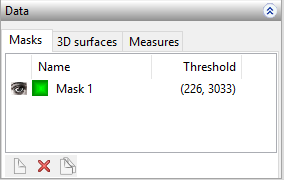
\includegraphics[scale=0.7]{../user_guide_figures/invesalius_screen/painel_mask_manager_en.png}
\caption{Data management}
\label{fig:volumetric_data}
\end{figure}

In each tab, there is a panel divided into rows and columns. The first column of each line determines the visualization status of the listed element. The "eye" icon activates or deactivates the masks, surface or measurement displayed. When one of these elements is being displayed, its corresponding icon (as shown in Figure~\ref{fig:disable_mask}) will also be visible.

\newpage

\begin{figure}[!htb]
\centering
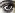
\includegraphics[scale=0.9]{../user_guide_figures/invesalius_screen/eye.jpg}
\caption{Icon indicating the elements visibility}
\label{fig:disable_mask}
\end{figure}

Some operations may be performed with the data. For instance, to remove one element, first select its name, as shown in Figure~\ref{fig:selected_mask}. Next, click in the shortcut shown in Figure~\ref{fig:delete_data}.

\begin{figure}[!htb]
\centering
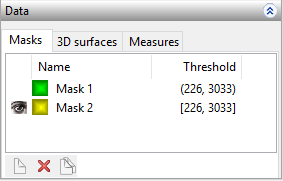
\includegraphics[scale=0.7]{../user_guide_figures/invesalius_screen/painel_selected_mask_en.png}
\caption{Data selected}
\label{fig:selected_mask}
\end{figure}


\begin{figure}[!htb]
\centering

\includegraphics[scale=0.8]{../user_guide_figures/icons/data_remove.png}
\caption{Remove data}
\label{fig:delete_data}
\end{figure}

To create a new mask, surface or measurement, click on the shortcut shown in Figure~\ref{fig:new_data}, provided that the corresponding tab is open.

\begin{figure}[!htb]
\centering

\includegraphics[scale=0.8]{../user_guide_figures/icons/data_new.png}
\caption{New data}
\label{fig:new_data}
\end{figure}

To duplicate data, select data to be duplicated and click in the shortcut shown in Figure~\ref{fig:duplicate_data}.

\begin{figure}[!htb]
\centering

\includegraphics[scale=0.8]{../user_guide_figures/icons/data_duplicate.png}
\caption{Duplicate data}
\label{fig:duplicate_data}
\end{figure}

\newpage

\section{Masks}

In the Name column, the mask’s color and name are shown. The \textbf{Threshold} column shows the value range used to create the mask. Figure~\ref{fig:volumetric_data} shows an example.

\section{3D Surface}

In the \textbf{Name} column, the surface’s color and name are shown. The \textbf{Volume} column shows the total surface volume. Finally, the \textbf{Transparency} column indicates the level of transparency for use for surface visualization. Figure~\ref{fig:surface_manager} shows an example.

\begin{figure}[!htb]
\centering
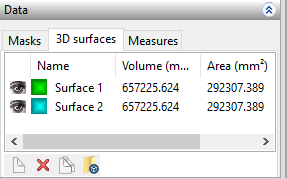
\includegraphics[scale=0.7]{../user_guide_figures/invesalius_screen/painel_volumetric_measures_en.png}
\caption{Surface manager}
\label{fig:surface_manager}
\end{figure}

\subsection{Import surface}

We can also import STL, OBJ, PLY or VTP (VTK Polydata File Format) files into an active InVesalius project. To do so, click in the icon shown in Figure~\ref{fig:import_stl}, select the format of the corresponding file, (Figure~\ref{fig:import_surface}) and click Open.

\begin{figure}[!htb]
\centering

\includegraphics[scale=0.8]{../user_guide_figures/icons/load_mesh.png}
\caption{Shortcut to import surface }
\label{fig:import_stl}
\end{figure}

\begin{figure}[!htb]
\centering
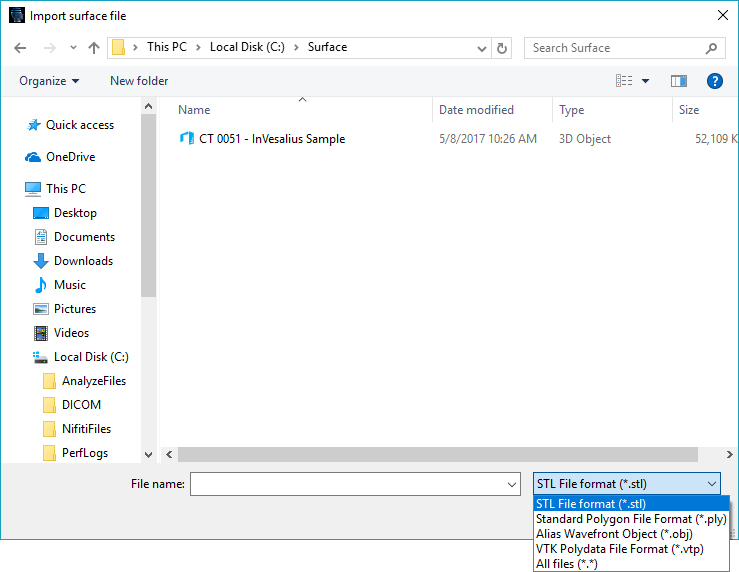
\includegraphics[scale=0.4]{../user_guide_figures/invesalius_screen/import_surface_en.png}
\caption{Window to import surface}
\label{fig:import_surface}
\end{figure}

\newpage


\section{Measurements}

The tab Measurements shows the following information. \textbf{Name} indicates the color and measurement name. \textbf{Local} indicates where the measurement was taken (image axial, coronal, sagital or 3D), and \textbf{Type} indicates the type of measurement (linear or angular). Finally, \textbf{Value} shows the measurement value. Figure~\ref{fig:manager_mensuares} illustrates the \textbf{Measurements} tab.

\begin{figure}[!htb]
\centering
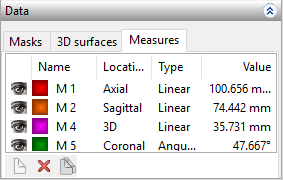
\includegraphics[scale=0.7]{../user_guide_figures/invesalius_screen/painel_measures_manager_en.png}
\caption{Data management}
\label{fig:manager_mensuares}
\end{figure}

